\begin{flushleft}

Der wichtigste Punkt war es nun eine lauffähige Schnittstelle zwischen ROS2 und einer Webanwendung herstellen zu können.
Für schnelles prototyping bietet die Open Source Robotic Foundation (OSRF) vorkonfigurierte Docker Container, in jeder beliebigen ROS Version, an.
Hierzu muss nur Docker Compose auf dem Rechner installiert sein, und ein fertiges Image kann sogleich erstellt werden.
%Um beispielsweise ein ROS2 Image mit der Foxy Fitzroy Version zu installieren, muss folgender Befehl ausgeführt werden. 
Für ein fertiges ROS Image mit der Foxy Fitzroy Version kann mit dem \textit{docker pull} [\ref{frontend_install}] Befehl installiert werden. 
% \begin{lstlisting}[language=bash]
%     docker pull osrf/ros:foxy-desktop 
% \end{lstlisting}

% \textit{foxy-desktop} kann hier mit jeder anderen beliebigen Version ausgetauscht werden. Mehr Informationen hierzu findet man im entsprechenden Docker Hub: 
% \begin{lstlisting}
%     https://hub.docker.com/r/osrf/ros/
% \end{lstlisting}

Da ROS Nodes über TCP/UDP Sockets kommunizieren, muss nun eine Brücke geschaffen werden, um Daten mit dem Web-Browser austauschen zu können.
Hier schafft das \cite[Rosbridge]{rosbridgepackage} Paket Abhilfe, in dem es einen Websocket erstellt, welcher in allen gängigen Web-Browsern unterstützt wird. Mit diesem Paket ist es nun möglich die bekannten Publish- und Subscribe-Funktionalitäten der ROS-Umgebung zu nutzen.
In der Abbildung \ref{fig:rosbridge_chain} wird die eben beschriebene Kommunikation vereinfacht dargestellt, sodass nun mehrere ROS Nodes mit dem Browser interagieren können.
\begin{figure}[h!]
    \centering
    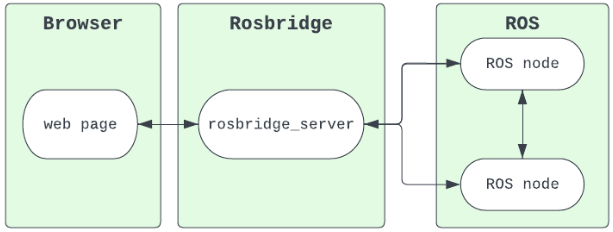
\includegraphics[width=0.8\textwidth]{imgs/web/rosbridge_chain.png}
    \caption{Rosbridge Kommunikation \cite{foxyglove_rosbridge_tut}}
    \label{fig:rosbridge_chain}%
\end{figure}
Die \textit{Rosbridge} kann ganz einfach über den apt-Paketmanager installiert werden.



% TODO Anhang Anleitung hinzufügen
Für eine genaue Anleitung um die \textit{Rosbridge} lauffähig zu bekommen, wird auf den Anhang verwiesen [\ref{frontend_install}].

Im nächsten Schritt wird eine einfache Webanwendung gebaut, die mit Hilfe der \textit{roslibjs} Bibliothek nun mit der \textit{Rosbridge} kommuniziert und Daten austauscht. 
Hierzu wird eine simple HTML-Seite erstellt und \textit{roslibjs} inkludiert. 

% \begin{lstlisting}[language=html]
% //Inkludierung und Quelle in HTML
% <script 
%     type="text/javascript" 
%     src="http://static.robotwebtools.org/roslibjs/current/roslib.min.js">
% </script> 


% \end{lstlisting}

% TODO Anhang Anleitung hinzufügen
Wenn nun die \textit{Rosbridge} erfolgreich in der ROS-Umgebung, in diesem Fall innerhalb des Docker Containers unseres Prototypens, gelauncht wurde, kann man sich mit einem Javascript-Objekt eine Verbindung zu dem Websocket aufbauen.
Hierzu wird die IP-Adresse des Docker-Containers mit dem Port 9090 benötigt.
Mit der URL \textit{ws://171.17.0.3:9090} haben wir uns beispielsweise in unserer Anwendung verbunden.
Ist die Verbindung erfolgreich hergestellt, können Publisher und Subscriber an das Objekt angebunden werden.
%Ausführliche Erklärungen und Code Beispiele sind im Anhang nachzulesen. (fehlt noch..)

Nachdem eine simple Schnittstelle zwischen ROS2 und einem Web-Browser erfolgreich hergestellt wurde, wird es im Folgenden um die Umsetzung der React-App gehen. 




\end{flushleft}